\documentclass[border=12pt]{standalone}
\def\pgfsysdriver{pgfsys-dvisvgm.def}
\usepackage[dvisvgm]{xcolor}
\usepackage{xeCJK}
\setCJKmainfont{HaranoAjiGothic-Regular.otf}[BoldFont=HaranoAjiGothic-Bold.otf]
\setCJKsansfont{HaranoAjiGothic-Regular.otf}[BoldFont=HaranoAjiGothic-Bold.otf]
\usepackage{amsmath,amssymb,tikz,lmodern}
\usetikzlibrary{arrows.meta,positioning,calc,fit,backgrounds}
\renewcommand{\familydefault}{\sfdefault}
\definecolor{ink}{HTML}{25322F}
\definecolor{green}{HTML}{246657}
\definecolor{tint}{HTML}{EEF4F0}
\definecolor{soft}{HTML}{C6D2CC}
\definecolor{muted}{HTML}{52615B}
\newif\ifJapanese
\newcommand{\Tx}[2]{\ifJapanese #1\else #2\fi}
\newcommand{\Eff}{\overline{\operatorname{Eff}}}
\newcommand{\heading}[3]{{\color{green}\bfseries #1\quad\Tx{#2}{#3}}\\[5pt]}
% A white rectangle makes the complete citation label clickable, including spaces.
\newcommand{\refurl}[2]{\special{dvisvgm:raw <a xlink:href="#1" target="_blank" rel="noopener noreferrer">}{\setlength{\fboxsep}{0pt}\colorbox{white}{\color{green}\underline{\strut #2}}}\special{dvisvgm:raw </a>}}
\newcommand{\refedge}[3]{\refurl{\csname source#1\endcsname\string##page=#2}{#3}}
\newcommand{\SF}[2]{\refedge{sf}{#1}{#2}}
% GitHub's file preview does not support PDF page fragments.
\newcommand{\LA}[2]{\refurl{\sourcela}{#2}}
\newcommand{\Sch}[2]{\refedge{sch}{#1}{#2}}
\newcommand{\PS}[2]{\refedge{ps}{#1}{#2}}
\tikzset{
 card/.style={draw=soft,fill=white,rounded corners=2pt,align=left,text=ink,font=\fontsize{10.5}{14}\selectfont,inner xsep=12pt,inner ysep=10pt,text width=14.4cm},
 half/.style={card,text width=6.45cm,minimum height=2.05cm},
 result/.style={card,draw=green,fill=tint,line width=.9pt},
 reason/.style={align=left,text=muted,font=\fontsize{9}{12}\selectfont,inner sep=0pt,text width=12.7cm},
 branchreason/.style={reason,text width=5.95cm},
 edge/.style={-{Stealth[length=2.4mm]},draw=green,line width=1pt},
 wire/.style={draw=green,line width=1pt},
}
% Keep the arrow in a dedicated left gutter; explanations never cover it.
\newcommand{\flow}[3]{
 \coordinate (#2-from) at ($(#1.south)+(-6.9,0)$);
 \coordinate (#2-to) at ($(#2.north)+(-6.9,0)$);
 \draw[edge] (#2-from)--(#2-to);
 \node[reason,anchor=west] (#2-reason) at ($(#2-from)!.5!(#2-to)+(.55,0)$) {#3};
}

\Japanesefalse
\newcommand{\sourcesf}{https://raw.githubusercontent.com/openai/math/adc7f1241b42e322a6451854ab7e4b4c146bf78a/preprints/Schnell-fiber-spaces-and-good-canonical-models-September-24-2026/paper.pdf}
\newcommand{\sourcela}{https://github.com/openai/math/blob/adc7f1241b42e322a6451854ab7e4b4c146bf78a/preprints/Log-abundance-in-characteristic-zero-September-24-2026/paper.pdf}
\newcommand{\sourcesch}{https://arxiv.org/pdf/2202.01295v1}
\newcommand{\sourceps}{https://arxiv.org/pdf/1405.6125v2}
\begin{document}
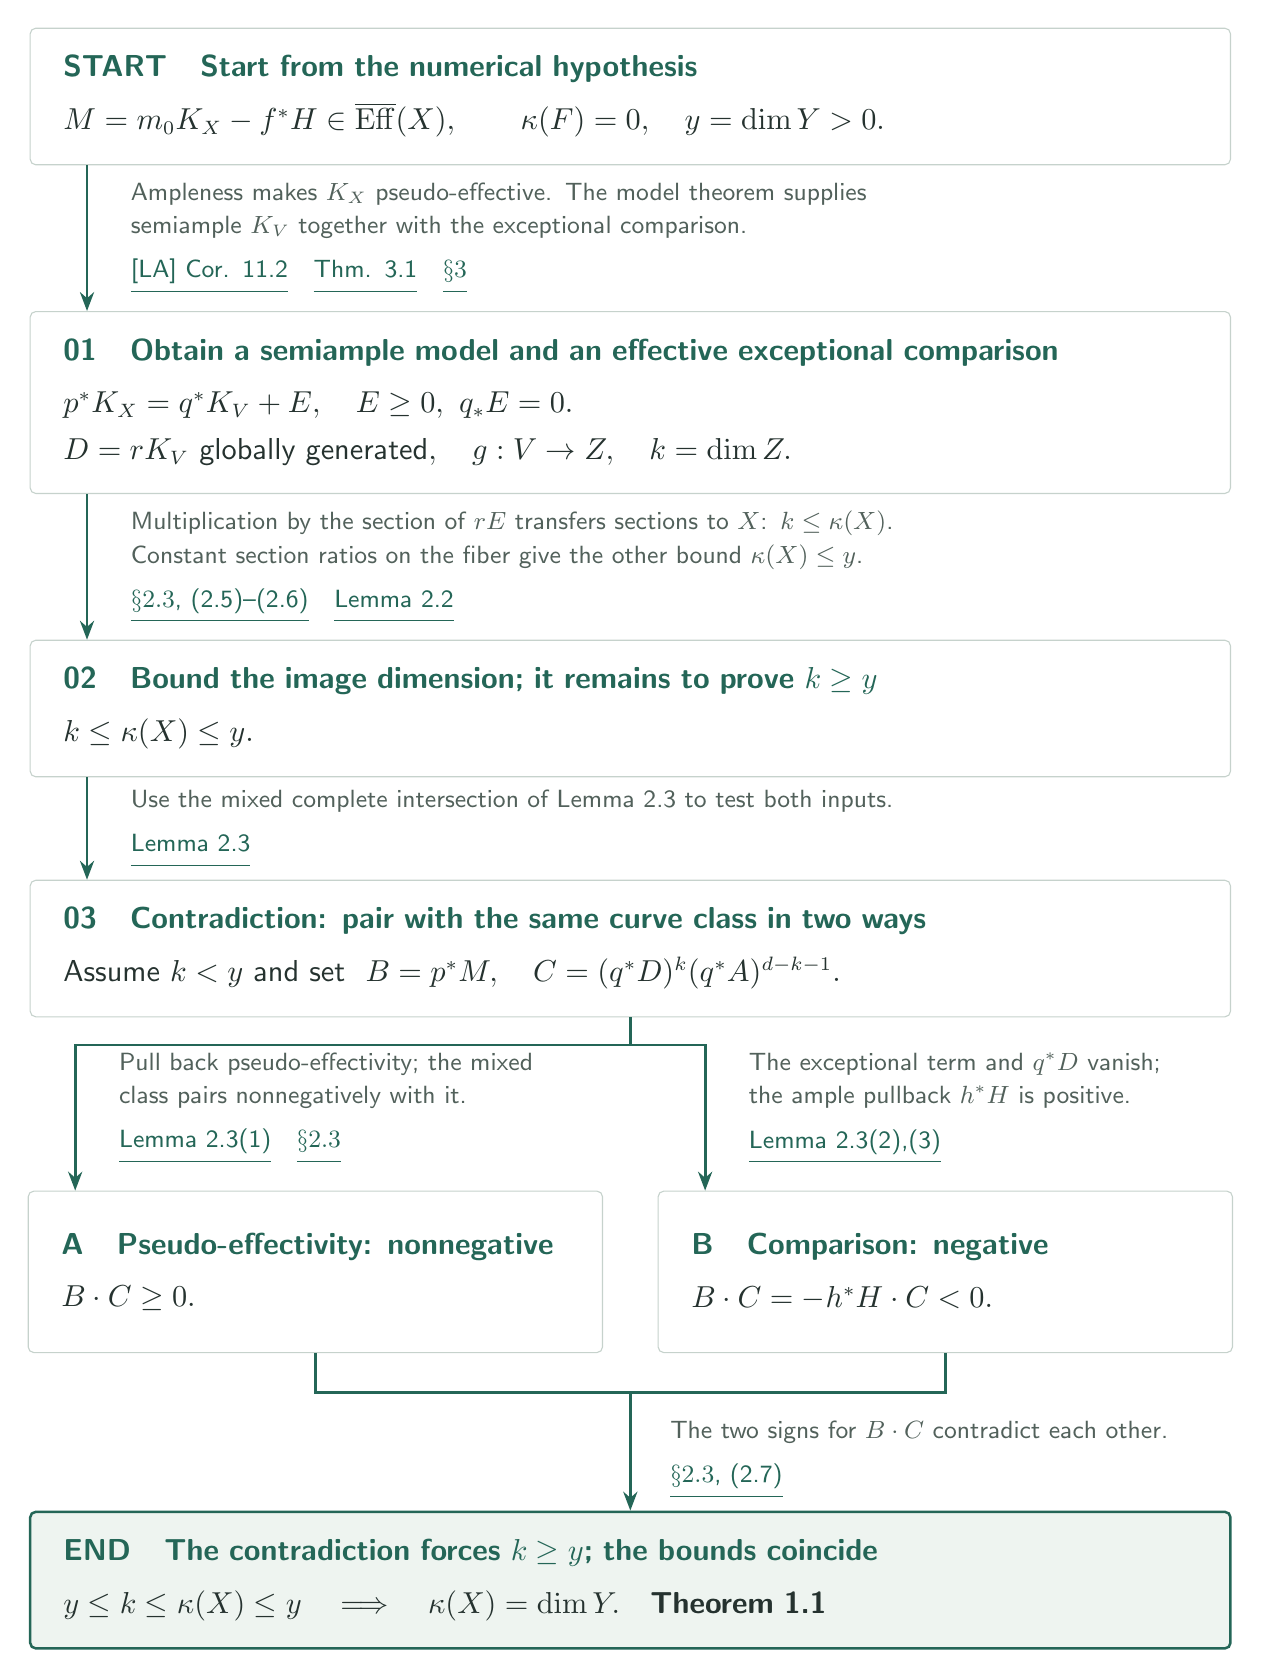
\begin{tikzpicture}
\node[card] (input) {\heading{START}{数値的仮定から出発する}{Start from the numerical hypothesis}
$M=m_0K_X-f^*H\in\Eff(X),\qquad \kappa(F)=0,\quad y=\dim Y>0.$};
\node[card,below=1.85cm of input] (model) {\heading{01}{半豊富なモデルと、有効な例外因子の比較式を得る}{Obtain a semiample model and an effective exceptional comparison}
$p^*K_X=q^*K_V+E,\quad E\ge0,\ q_*E=0.$\\[3pt]
$D=rK_V\text{ globally generated},\quad g:V\to Z,\quad k=\dim Z.$};
\flow{input}{model}{\Tx{$H$ の豊富性より $K_X$ は擬有効。モデル存在定理から、\\半豊富な $K_V$ と有効な例外因子の比較式を得る。}{Ampleness makes $K_X$ pseudo-effective. The model theorem supplies\\semiample $K_V$ together with the exceptional comparison.}\\[4pt]
\LA{73}{[LA] Cor. 11.2}\quad\SF{7}{Thm. 3.1}\quad\SF{8}{$\S3$}}
\node[card,below=1.85cm of model] (bounds) {\heading{02}{像の次元をはさむ。残る目標は $k\ge y$}{Bound the image dimension; it remains to prove $k\ge y$}
$k\le\kappa(X)\le y.$};
\flow{model}{bounds}{\Tx{$rE$ の標準切断を掛けて切断を $X$ へ移すと、$k\le\kappa(X)$。\\一方、ファイバー上の切断比は定数なので $\kappa(X)\le y$。}{Multiplication by the section of $rE$ transfers sections to $X$: $k\le\kappa(X)$.\\Constant section ratios on the fiber give the other bound $\kappa(X)\le y$.}\\[4pt]
\SF{6}{$\S2.3$, (2.5)--(2.6)}\quad\SF{4}{Lemma 2.2}}
\node[card,below=1.3cm of bounds] (test) {\heading{03}{背理法：同じ曲線類で、二つの交点数評価を比べる}{Contradiction: pair with the same curve class in two ways}
\Tx{$k<y$ と仮定し、}{Assume $k<y$ and set }
$B=p^*M,\quad C=(q^*D)^k(q^*A)^{d-k-1}.$};
\flow{bounds}{test}{\Tx{Lemma 2.3 の混合完全交差を使い、擬有効性とモデルの比較式を試す。}{Use the mixed complete intersection of Lemma 2.3 to test both inputs.}\\[4pt]\SF{5}{Lemma 2.3}}
\node[half,below=2.2cm of test.south,anchor=north,xshift=-4cm] (nonnegative) {\heading{A}{擬有効性からは、非負}{Pseudo-effectivity: nonnegative}
$B\cdot C\ge0.$};
\node[half,below=2.2cm of test.south,anchor=north,xshift=4cm] (negative) {\heading{B}{比較式からは、負}{Comparison: negative}
$B\cdot C=-h^*H\cdot C<0.$};
\draw[wire] (test.south)--++(0,-.35) coordinate (fork);
\draw[edge] (fork)-| ($(nonnegative.north)+(-3.05,0)$);
\draw[edge] (fork)-| ($(negative.north)+(-3.05,0)$);
\node[branchreason,anchor=west] (positive-reason) at ($(nonnegative.north)+(-2.5,1.05)$) {\Tx{擬有効性を引き戻し、$C$ との\\交点数が非負になる性質を使う。}{Pull back pseudo-effectivity; the mixed\\class pairs nonnegatively with it.}\\[4pt]\SF{5}{Lemma 2.3(1)}\quad\SF{7}{$\S2.3$}};
\node[branchreason,anchor=west] (negative-reason) at ($(negative.north)+(-2.5,1.05)$) {\Tx{例外項と $q^*D$ の寄与は $0$、\\底の豊富因子 $h^*H$ の寄与は正。}{The exceptional term and $q^*D$ vanish;\\the ample pullback $h^*H$ is positive.}\\[4pt]\SF{5}{Lemma 2.3(2),(3)}};
\node[result,below=2cm of nonnegative.south,anchor=north,xshift=4cm] (goal) {\heading{END}{矛盾により $k\ge y$。上下界が一致して主定理を得る}{The contradiction forces $k\ge y$; the bounds coincide}
$y\le k\le\kappa(X)\le y\quad\Longrightarrow\quad\kappa(X)=\dim Y.$\quad\textbf{Theorem 1.1}};
\coordinate (join) at ($(goal.north)+(0,1.5)$);
\draw[wire] (nonnegative.south)|-(join);
\draw[wire] (negative.south)|-(join);
\draw[edge] (join)--(goal.north);
\node[reason,text width=6.7cm,anchor=west] (goal-reason) at ($(goal.north)+(.5,.65)$) {\Tx{同じ $B\cdot C$ が非負かつ負となり矛盾。}{The two signs for $B\cdot C$ contradict each other.}\\[4pt]\SF{7}{$\S2.3$, (2.7)}};
\end{tikzpicture}

\end{document}
